\chapter{Annexe - Source du rayonnement}
Ce paragraphe \textbf{hors-matière} reprend les idées du cours de manière plus détaillée quant à la source du rayonnement électromagnétique. Il traite de l'intuition qui se cache derrière les champs rayonnés : il se réfère aux lectures supplémentaires disponibles \dots \\ 
A l'instar du concept de particule chargée au repos dans un référentiel galiléen classique créant un champ électrique statique et à l'instar du même genre de particule mais cette fois-ci en mouvement à vitesse constante uniforme générant un champ magnétique, lorsque la particule est accélérée il se développe alors ce que nous appelons un champ rayonné : une onde électromagnétique. Ce champ rayonné intégrera donc un couplage entre champ magnétique et champ électrique. \\
Nous nous proposons ici d'expliquer brièvement en quoi, lorsqu'une charge est accélérée, un phénomène de radiation apparaît. Il est tout d'abord nécessaire de s'imaginer un champ électrique statique associé à une charge au repos. Admettons que pour une certaine raison, elle soit accélérée uniformément selon la direction $\hat{x}$ du référentiel considéré avec une intensité $a$ pendant un temps $\tau$ à partir de $t = 0$. Après, pour $t>\tau$, l'accélération cesse et la particule continue son bonhomme de chemin à une allure constante $v = a\,\tau$ selon $\hat{x}$. A vitesse constante, la particule développe non seulement un champ magnétique mais également un champ électrique non-plus statique mais en mouvement ; en vulgarisant quelque peu, "\textit{centré et attaché}" à la particule. En considérant les temps $t = 0$ et $t = \tau$, nous observons aisément que le champ électrique associé à la particule chargée n'est pas centré au même endroit : il a non seulement été projeté en avant suite au mouvement de la particule mais ce de manière plus rapide que la vitesse initiale constante de déplacement du champ électrique jusque là (accélération). Le développement suivi ici est donc valable pour toute accélération de la particule chargée : qu'importe sa vitesse initiale. Cependant, et c'est là où réside toute l'essence même du rayonnement, ce changement de \textit{centrage} ne s'opère pas de manière instantanée! La figure \ref{fig:yo} montre bien que "\textit{l'information physique}" se propage à vitesse finie ($c = \frac{1}{\sqrt{\epsilon\,\mu}} < \infty $) vers l'extérieur.\\ \\
En première approximation, nous pouvons tracer des traits entre les lignes du nouveau champ électrique s'établissant progressivement et un champ électrique issu de temps antérieurs. Nous pouvons nous figurer que lorsque l'accélération cesse, tous ces changements cessent également et aucune "\textit{information}" supplémentaire sur la nature  du champ ne se propage. Cette "\textit{information}" dont nous traitons depuis quelques lignes n'est rien d'autre qu'un champ électrique rayonné qui vient se superposer au champ électrique latent afin que le champ électrique total résultant tende à se calquer vers un champ électrique plus actuel (comprendre : associé à la particule chargée en un temps postérieur). 
\begin{marginfigure}
	\centering
	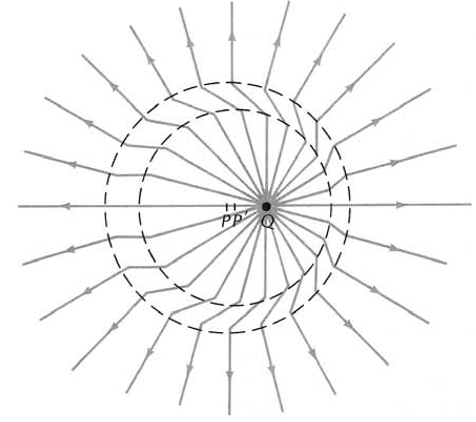
\includegraphics[height=4.3cm]{figure_ray.png}
	\caption{Illustration du changement de \textit{centrage} et propagation du signal (tirée des lectures complémentaires). Q est la position actuelle de la charge, P la position initiale. Entre P et P', la charge a subi une accélération, depuis, elle bouge à vitesse constante.}%Pas toute la description, 
	\label{fig:yo}
\end{marginfigure}

Sans rentrer dans les détails d'un développement mathématique fastidieux, forts de ce constat, nous pouvons avancer que l'évolution du champ rayonné en un point de l'espace $\vec{r}$ dépend non pas du temps actuel $t$ mais bien du temps $t' = t - \frac{|| \vec{r} - \vec{r}_{p} ||}{c}$ qu'il était lorsque l'accélération instantanée (menant à la propagation d'un front d'onde comme sur la figure \ref{fig:yo}) tint lieu. En effet, il faut tenir compte du déphasage temporel $\frac{||\vec{r} - \vec{r}_{p} ||}{c}$ lié au temps mis par le front d'onde pour arriver en $\vec{r}$ depuis $\vec{r}_{p}$ (position où l'accélération a été subie).

Aussi, intuitivement, nous accepterons pour la suite du document que l'amplitude du champ rayonné est directement proportionnelle à l'accélération subie. En effet, admettons que celle-ci soit minuscule : en repartant de notre scénario initial, la particule chargée avancera à peine et ce de manière très lente, le champ rayonné afin d'homogénéiser l'espace entier par rapport à un nouveau champ électrique issu de la particule s'étant déplacée sera de très faible amplitude car peu de choses auront réellement changé. De plus, si jamais nous avions considéré une accélération dans le sens opposé, il est clair que le schéma de la figure \ref{fig:yo} aurait simplement subi une symétrie axiale.\\ Désormais, il va nous falloir admettre un postulat ; confirmé par la figure \ref{fig:yo} si nous regardons dans la direction de l'accélération. Il s'agit d'observer que seule la composante orthogonale de l'accélération en $t'$ par rapport à la position $\vec{r}$ considérée entraîne un rayonnement. Cet effet est illustré à la figure \ref{fig:yo2} directement prélevée des slides du cours. A la figure \ref{fig:yo}, nous imaginons déjà qu'aucun champ rayonné n'apparaît dans la direction $\hat{x}$ puisqu'il n'y a pas de déformation de la ligne de champ dans cette même direction.

Enfin, puisque la puissance du signal (champ électrique) se propageant doit être conservée et qu'il se propage dans toutes les directions \footnote{Nous verrons qu'il faut être prudent en disant cela : certaines directions se verront doter d'une propagation de champ rayonné d'amplitude nulle. Il est ici juste nécessaire de saisir les idées sous-jacentes.}, il faut savoir que l'intensité ([$W/m^{2}$]) du champ rayonné sera proportionnelle à $\frac{1}{|| \vec{r} - \vec{r}_{p} ||^{2} }$ puisque le front d'onde décrit successivement des boules centrées en $\vec{r}_{p}$ d'enveloppe de surface évoluant avec le carré du rayon. Attendu que, comme nous avons pu le découvrir, l'intensité est directement liée au carré de l'amplitude du champ électrique associé ; cette dernière sera proportionnelle à $\frac{1}{||\vec{r} - \vec{r}_{p}||}$ = $r'$ .
